\documentclass[a4paper,10pt]{article}

\usepackage[a4paper, total={6in, 9in}]{geometry}
\usepackage[utf8]{inputenc}
\usepackage{amsmath}
\usepackage{amsfonts}
\usepackage{graphicx}
\usepackage[ruled,vlined]{algorithm2e}
\usepackage{hyperref}
\usepackage{cleveref}
\usepackage{color}
\usepackage{subcaption}

\author{Harry Tzovas}

\definecolor{blue1}{RGB}{44,127,184}

\newcommand{\wave}{$\mathcal{WAVE}$ }

\newcommand{\bull}{$\bullet$}
\newcommand{\red}[1]{{\color{red}{#1}}}
\newcommand{\blue}[1]{{\color{blue1}{#1}}}
\newcommand{\mz}{\mathbb{Z}}
\newcommand{\quot}[1]{``#1''}
\newcommand{\km}{$k$-means}
\newcommand{\todo}[1]{{\red{TODO}}: #1}
\newcommand\noIndent[1]{
  \par\vbox{\parbox[t]{\linewidth}{#1}}
}

\graphicspath{{/home/harry/wave/figures/}{../figures/}}


\begin{document}

This is meant as a place to document problems and TODOs, possible solutions and ideas and, when some
idea is implemented, what are the results.

\section*{PE renumbering}
Given a partition, we want to redistribute data based on that. A function for this  exists in
aux::redistributeFromPartition. Theoretically, it can happen that PE $P_j$ have local points that belong
to other PEs, that is, $\text{localPart}(i)\neq j,\; \forall i\in P_j$. So it will send local data and receive new.

\paragraph*{Idea:}  Before redistribution, every PE goes over its local points and counts how many points
are belong to each block. Then, if for PE $P_j$, the majority of its local points belong to block $k$,
we will renumber block $k$ to $j$. This way, $P_j$ will keep as many points as possible. 

The problem is that many PEs can request for different renumbering of the same block. 
For example, in PE $P_0$ the majority of its local points, say $30\%$ belong to block $3$ 
but also, the majority of points in $P_1$ belongs also block $3$ with $40\%$ of the points in $P_1$. 
So $P_0$ want the renumbering 3 to 0 and $P_1$ the renumbering
3 to 1. For that, every PE claims a new label and this are globally summed to avoid conflicts.
For every conflicting request, we accept the one with the largest weight. In the example above,
we will pick 3 to 1 since $P_1$'s weight is 0.4 and $P_0$'s is 0.3. The PE that did not get claimed
id will request another id in the next round. If all wanted ids are taken, it will pick one
at random. We repeat until every PEs has picked an id.

\paragraph*{Result:} The idea is implemented in aux::redistributeFromPartition. For random partitions
it works, but it does not do anything for k-means. That is, every PE claims its own id.

After the hilbert curve sorting, every PE has points that are local, i.e., $\forall i \in P_j,
\text{localPart}(i)=j$. After k-means, PEs can have points from different blocks but usually
the majority of their local points still belong to them. For the renumbering to work, at least
2 PEs must claim a different id but this rarely happens (I noticed that most blocks still own
$50-70\%$ of their points after k-means). This makes sense. I did not test that in detail, but in
a few graph I tried, every PE claimed its own id, so no renumbering occurred. Maybe with smaller 
blocks this can have some effect.



\section*{Hierarchical k-means results}

In some case, a block can be completely inside another one.

\begin{figure}
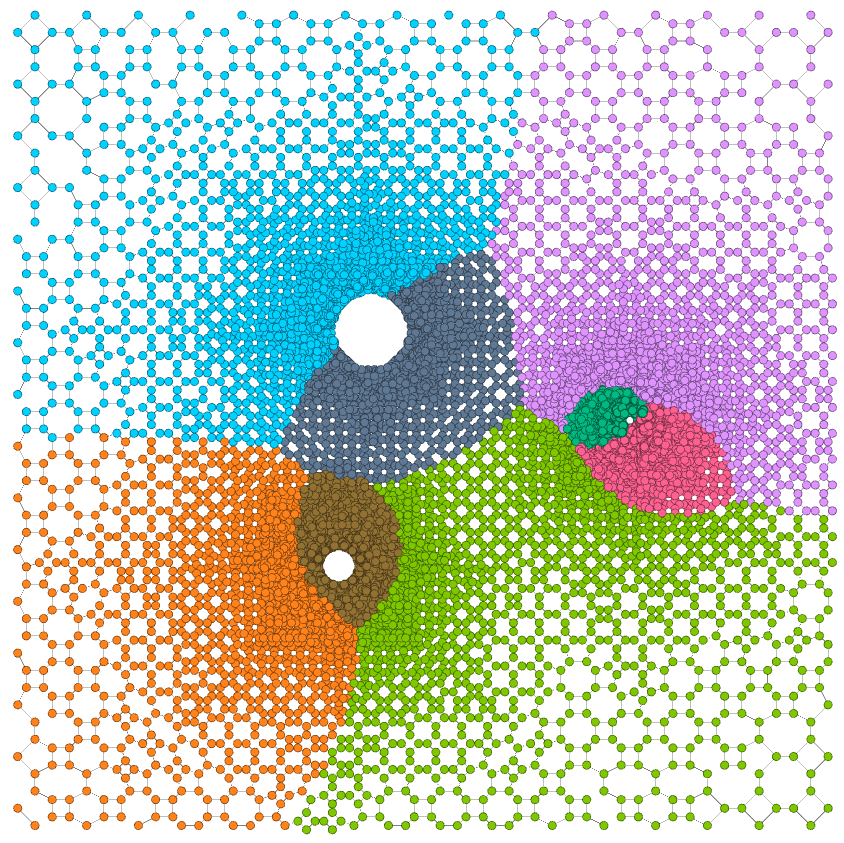
\includegraphics[scale=0.3]{slowrot_KMeans_k8.png}
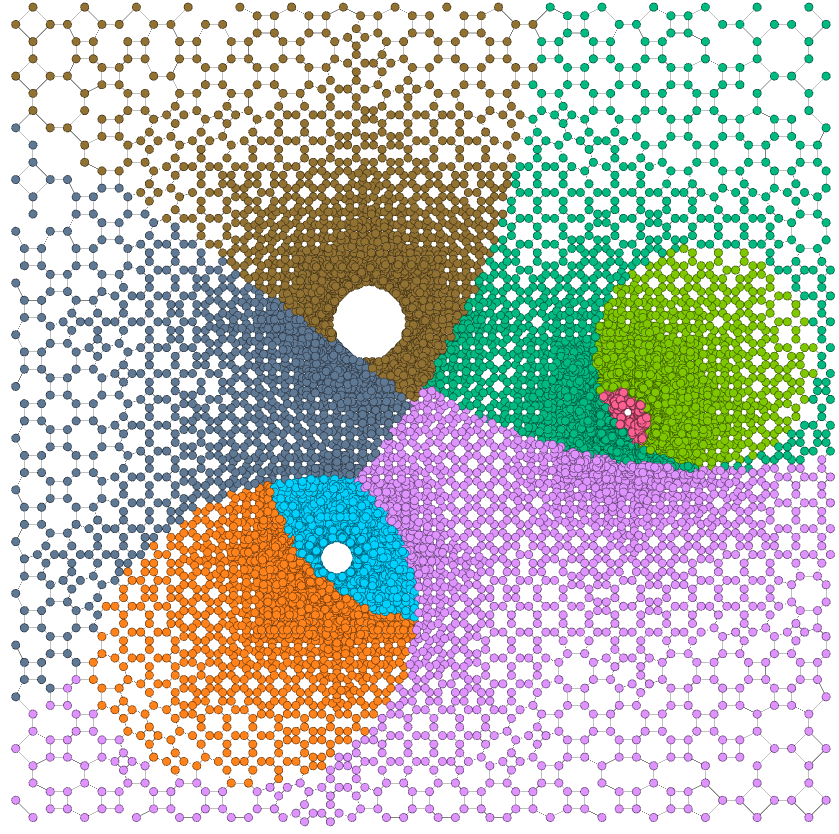
\includegraphics[scale=0.3]{slowrot_HKMeans_k8.png}
\caption{Graph slowrot0 partitioned  with k-means and the hierarchical version }.
\end{figure}


\begin{figure}
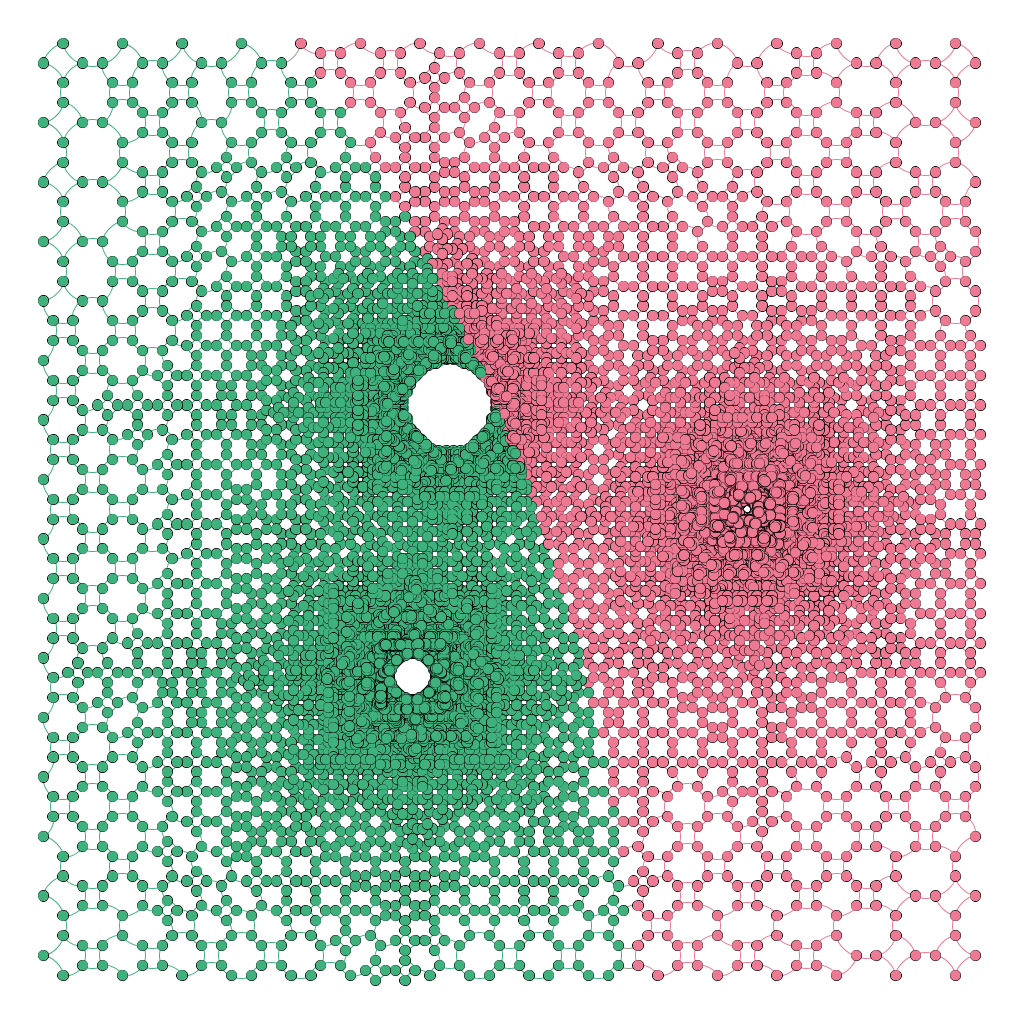
\includegraphics[scale=0.2]{slowrot_RecursiveKMeans_k2}
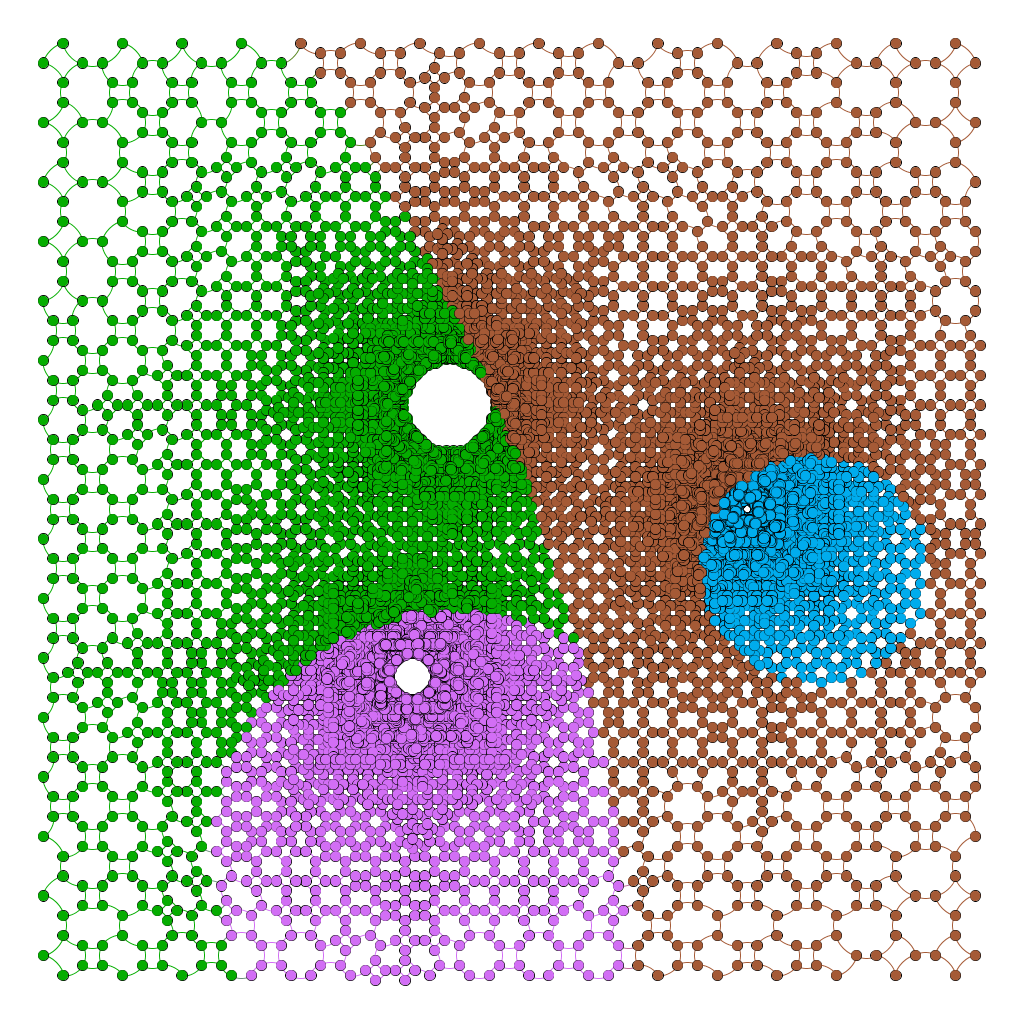
\includegraphics[scale=0.2]{slowrot_RecursiveKMeans_k4}

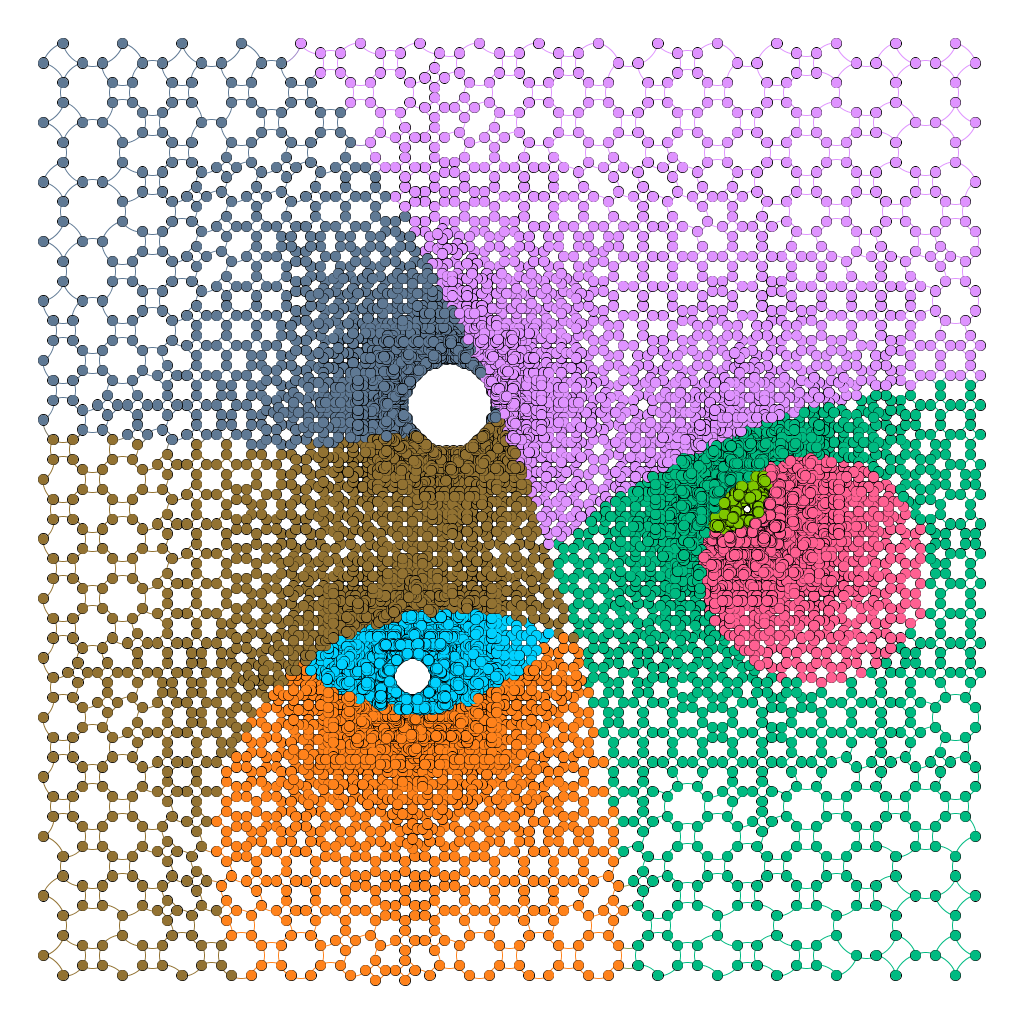
\includegraphics[scale=0.2]{slowrot_RecursiveKMeans_k8}
\caption{Graph slowrot0 partitioned recursively into 8 blocks. }
\end{figure}



\section*{Get communication graph in parallel}

We want to build the communication/block graph $G_c$ given the input, application graph $G_a$ and a
partition into $k$ blocks. Notice that $V(G_c)=k$, edges $E(G_c)$ are weighted and every PE owns some subset 
of $E(G_c)$. Even more,
edges can be divided among PEs, for example, PE 1 can own edge $(4,5)$ with weight $10$ and the same
edge can be present in other PEs with different weights. The actual weight of the edge $(4,5)$ is the
sum of the weights.

\paragraph*{One solution} is to create the complete graph of size $k^2$. Every PE sets the weights of the edges that
it owns. Then, with a global sum operation the edge weights are added and scattered back to all PEs.
This is problematic for large $k$.
Maybe we could avoid the quadratic space if we know how many edges $G_c$ has. But this is not easy either.

\paragraph*{Another} way is that every PE sends its own edges and weights to a root PE, the root PE gather all the
edges, constructs the block graph and scatters the graph back to all PEs.

\paragraph*{Update, 19/03/19:} The parallel version works now. One possible problem is that we need to create
an array with the edges in one root PE where we gather all edges from all PEs. This arrays can have 
big size since some edges of $G_c$ exist in many PEs. For example, if blocks 4 and 5 have a boundary 
and are present in 4 PEs, then the edge $(4,5)$ will appear 4 times in this array. Still, this
is much better than the quadratic size. One solution can be to have a communication pattern like
the global sum and at every step edge weights are summed and duplicates are eliminated.

TODO: run a benchmark to see if and how faster this is.

\paragraph*{A possibly} better approach is not everything to one PE but consider each PE responsible
for some rows/vertices of the block graph. The, every PE, for every local edge will send the information 
to the responsible PE for this row/vertex. Then, the PE will add up the edges they received and
broadcast everything back. This is less centralized but may trigger more complicated communication 
patterns. If the block graph needs to be replicated, the several broadcast at the last step may
cause congestion.

\paragraph*{In parallel}: The communication graph is used to create the communication schedule
based on the edge coloring of the graph. The edge coloring can be also computed in parallel
avoiding the explicit construction of the communication graph. Not computing the communication
is essential for higher scalability since, for high numbers of PEs, it is a possible bottleneck although
this should be investigated further. Few new, relevant papers are:
\begin{enumerate}
\item \href{https://dl.acm.org/citation.cfm?id=3188906}
{Deterministic distributed edge-coloring with fewer colors}

\item \href{https://dl.acm.org/citation.cfm?id=3175473}
{The complexity of distributed edge coloring with small palettes}

\item \href{https://dl.acm.org/citation.cfm?id=2722155}
{$(2\Delta -1)$-edge-coloring is much easier than maximal matching in the distributed setting}

\item \href{https://dl.acm.org/citation.cfm?id=282804}
{Near-optimal, distributed edge colouring via the nibble method}

\end{enumerate}


\end{document}
